\documentclass[12pt]{article}
\usepackage{graphicx}
\graphicspath{{./images/}}
\title{Idee Arhitectură}
\author{Dumitru Marius-Vlad}
\date{\today}

\begin{document}
\maketitle

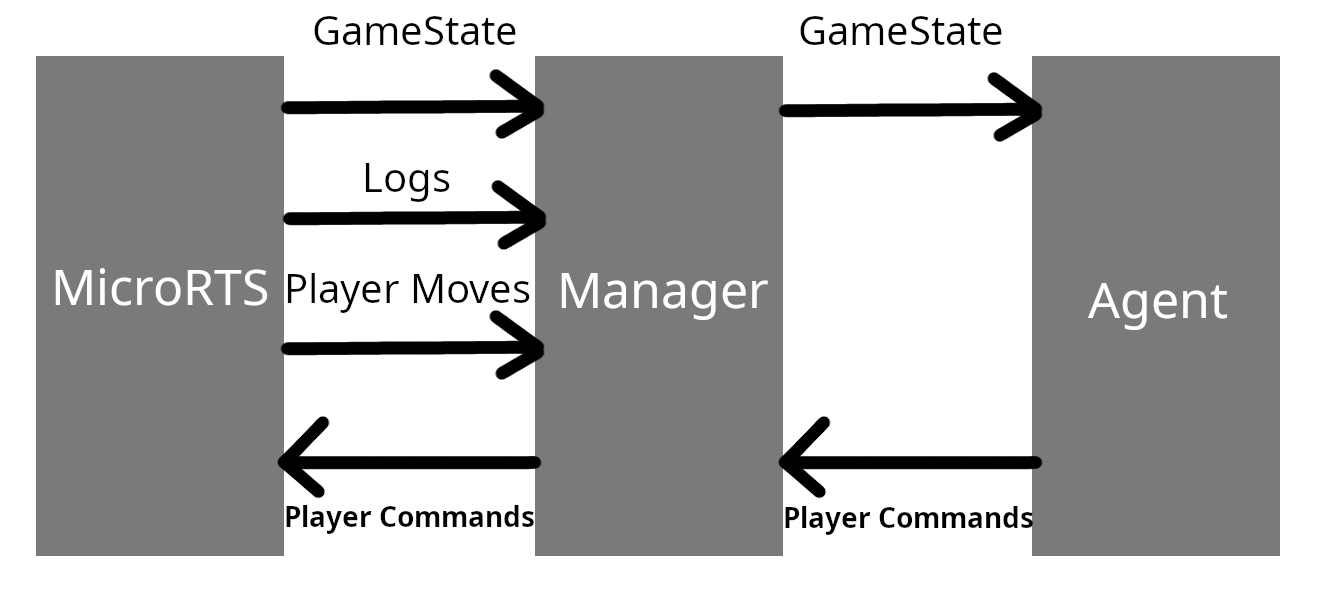
\includegraphics[scale=0.6]{Architecture_Idea_3Comp.png}

A existat o discuție, la un moment dat, despre posibilitatea implementării de servere private("private server"). Atunci am avut această idee de arhitecutră cu 3 componente principale.\\
Pe scurt, m-am gândit la o arhitectură generică, cu 3 componente principale: \textbf{jocul(MicroRTS)}, un \textbf{manager}, \textbf{agentul/agenții}.\\
Agentul/agenții să ruleze undeva în cloud ca să poată rula pe GPU, iar MicroRTS și Managerul să ruleze local, pe un calculator.\\
MicroRTS este sub forma unui fișier .jar, Managerul ar fi sub forma unuia sau mai multe pachete python, Agentul/Agenții ar fi sub forma unui jupyter notebook(+ eventuale pachete python).\\
Ar fi vorba despre o arhitectură tip \textbf{client-server}, unde Managerul ar fi serverul, iar clienții ar fi MicroRTS și Agentul/Agenții.\\
Task-urile fiecăruia(idei în mare):\\
\textbf{MicroRTS:}
\begin{itemize}
    \item Prin Visualizerul intern, să afișeze desfășurarea meciului: harta, unitățile playerilor pe hartă, ce fac unitățile pe hartă(move, attack, construct, etc.) în timp real. Doar așa pot vedea, vizual, meciul propriu-zis.
    \item Să primească comenzile agenților și să le execute(ex: P1 move unitate a la pozitia y, P2 attack cu unitatea b la pozitia y, etc), în același timp actualizând game state-ul.
    \item Să transmită GameState-ul (situația meciului - are structură internă care o descrie) către agent/agenți.
    \item Eventual să transmită niște log-uri și ordinea mutărilor(ca la șah, unde fiecare mutare, de la oricare jucător, este consemnată, în ordinea apariției). Nu cred că, acum, jocul are implementat suport pentru acest lucru. Putem renunța la acest aspect, dacă este cazul.
    \item Eventual să ofere posibilitatea să creez hărți noi. Jocul vine, din fabrică, cu un număr de hărți, dar mi-ar plăcea să am un fel de "Map Maker/Map Creator" unde îmi definesc hărțile: dimensiunea, nr. de jucători, geografia(tile-uri pe care nu mă pot pozitiona - ca niste ziduri/munți/ peste care nu pot trece), poziții ale unor unități/clădiri la începutul meciului - care mi-ar permite construcția diverselor scenarii.
\end{itemize}

\textbf{Managerul}:\\
\begin{itemize}
    \item Să pornească/oprească serverul la care se vor conecta jocul și agentul/agenții.
    \item Să primească de la agent/agenți comenzile pentru player și să le transmită, mai departe, la joc.
    \item Să primească de la joc game state-ul și să-l transmită mai departe către agent/agenți.
    \item Să primească log-urile/mutările de la joc (daca e cazul) și să le stocheze.
    \item Să citească configurația meciului/meciurilor și să comande "START GAME"/"START GAMES":\\
    Aici vine ideea de "servere private" despre care am discutat anterior.\\
    Ideea de "server privat clasic" știam că înseamnă, în acceptiunea clasică(Warcraft3/Starcraft Bood War, etc.) că oricare instanță a jocului poate deveni un server, la care se conectează alte instanțe ale jocului - clienții.\\
    Serverul este autoritar adică el configurează meciul(pe ce hartă se joacă, câți jucători, definește win rulez(cine reușește primul să elimine toate clădirile + unitățile inamice câștigă/ primul care farmează x gold + y wood / z whatever câștigă/ primul care rezistă x min în fața invaziei inamice câștigă/)), el poate banna pe oricine să nu se conecteze/ poate da kick oricui din meci, etc. Clienții se conectează la server, dau click pe butonul "Ready", iar la final(dup ce toată lumea a dat "Ready"), serveru dă "Start Game".\\
    Meciul pornește, se joacă, se termină.\\
    La final, colectează și afișează statistici: câștigători/pierzători, nr. unități pierdute, gold/wood farmat, upgrade-uri, etc.\\
    In acest proiect, managerul să facă lucruri similare, adică, să existe configurații predefinite de scenarii/batch-uri de meciuri/meciuri individuale - (1v1, capture the flag, move to pozition x, defend pozition, numărul de jucători, poziiții de start, etc.). Managerul să citească aceste informații să le trimită către agenți și joc, ei să își facă un setup inițial(când e gata să confirme cu un "I'm ready"), iar managerul să dea "Start Game".\\
    În timpul meciului/meciurilor/scenariilor, managerul să colecteze și să înregistreze ce se întâmplă. La final să aibă o statistică de genul: câștigători/pierzători, gold farmat, unități capturate etc. pe meci individual/ batch de meciuri/scenariu unic/ mai multe scenarii.\\
    Din datele colectate să pot extrage date statistice (grafice, tabele), pe care să le folosesc mai departe la îmbunătățirea modelelor/ prezentarea rezultatelor în lucrare.\\
    Știu că partea acesta este foarte incipientă, dar cam asta este ideea de bază - culesul de date de-a lunul unor scenarii diferite(pe mai multe seturi de meciuri) și agregarea lor în tabele și grafice pentru a putea trage concluzii.\\
    Eventual să am mai multe instanțe de joc-manager-agent, fiecare să ruleze diverse scenarii, să le las să-și facă bucătăria internă, iar la final, după ce s-au colectat toate datele, să văd un rezumat la ce sa întâmplat.
\end{itemize}

\textbf{Agentul/Agenți:}
\begin{itemize}
    \item Ei vor fi entitatea/entitățile care vor controla jucătorii.
    \item Sunt resposabili cu luarea deciziilor în funcție de ce gamestate primesc.
    \item Trebuie să hotărască ce acțiuni trebuie să facă ca să atingă un anumit scop predefinit(win condition-ul meciului).
    \item O dată ce sa hotărât ce să facă, trasmite acțiunea/acțiunile către manager care le transmite mai departe către joc. Playerul(playerii) "joacă" așa cum a dictat agentul și trimite feedback(gamestate sau poate gamestate + altceva) către manager care le trimite mai departe către agent.
    \item Practic aici este o buclă continuă Percepție $\rightarrow$ Decizie $\rightarrow$ Acțiune. După setup-ul inițial , sa dat "start joc", agentul primește gamestate(percepție), se gândește ce să facă (decizie), execută ceea ce a gândit (acțiune) $\rightarrow$ repeat. Asta fiind și bucla principală(main loop-ul) proiectului.
    \item Presupun că este nevoie de putere de procesare aici(deci de GPU), de aceea m-am gândit la rularea în cloud.
\end{itemize}



\end{document}